\documentclass[aspectratio=169,12pt,t]{beamer}

% --- Theme: Metropolis (modern, clean) ---
\usetheme[progressbar=frametitle,numbering=fraction,block=fill]{metropolis}

% --- Fira Sans font (install texlive-fonts-extra if missing) ---
\IfFileExists{FiraSans.sty}{\usepackage[sfdefault]{FiraSans}}{}

% --- Light background with warm accent ---
\definecolor{mDarkTeal}{RGB}{35,55,59}
\definecolor{mLightBrown}{RGB}{235,228,216}
\definecolor{mAccent}{RGB}{140,70,20}

\setbeamercolor{normal text}{fg=mDarkTeal,bg=white}
\setbeamercolor{alerted text}{fg=mAccent}
\setbeamercolor{frametitle}{bg=mDarkTeal,fg=white}
\setbeamercolor{progress bar}{fg=mAccent,bg=mLightBrown}
\setbeamercolor{title separator}{fg=mAccent}
\setbeamercolor{progress bar in head/foot}{fg=mAccent,bg=mLightBrown}
\setbeamercolor{progress bar in section page}{fg=mAccent,bg=mLightBrown}

% --- Packages ---
\usepackage[utf8]{inputenc}
\usepackage{amsmath,amssymb,amsthm}
\usepackage{mathrsfs}
\usepackage{tikz}
\usetikzlibrary{arrows.meta,positioning,calc,decorations.pathreplacing,shapes,patterns}
\usepackage{pgfplots}
\pgfplotsset{compat=1.18}

% --- TikZ diagram styles (shared across the series) ---
\tikzset{
  axisln/.style={-{Stealth[length=2.6mm]}, line width=0.8pt, gray!75},
  curveln/.style={line width=1.6pt, line cap=round, line join=round},
  projln/.style={dash pattern=on 2.6pt off 2pt, line width=0.7pt},
  guide/.style={-{Stealth[length=2.6mm,width=2.2mm]}, line width=1.1pt},
  vec/.style={-{Stealth[length=3mm,width=2.4mm]}, line width=1.4pt},
  chord/.style={line width=1.2pt, line cap=round, line join=round},
}
% point marker with a white halo: \dotpt{color}{(coord)}
\newcommand{\dotpt}[2]{%
  \fill[white] #2 circle (3.6pt);
  \fill[#1] #2 circle (2.4pt);
}
% open point marker: \opendotpt{color}{(coord)}
\newcommand{\opendotpt}[2]{%
  \fill[white] #2 circle (3.6pt);
  \draw[#1, line width=1pt] #2 circle (2.4pt);
}
% the sample curve used in several pictures: gamma(t) = (gx(t), gy(t)), 0 <= t <= 1
\newcommand{\gx}[1]{6.5*(#1)}
\newcommand{\gy}[1]{1.55+1.15*sin(400*(#1))}

% --- Semi-transparent white highlight for text on top of background images ---
\usepackage[most]{tcolorbox}

% Inline highlight: \hl{short text}
\newtcbox{\hl}{%
  nobeforeafter, tcbox raise base,
  colback=white, opacityback=0.6,
  colframe=white, opacityframe=0,
  sharp corners, boxsep=2pt, left=3pt, right=3pt, top=2pt, bottom=2pt%
}

% Block highlight: \begin{hlbox} ... \end{hlbox}  (multi-line, paragraphs, itemize)
% Optional argument accepts any tcolorbox key, e.g. [width=0.6\linewidth]
\newtcolorbox{hlbox}[1][]{%
  enhanced, breakable,
  colback=white, opacityback=0.6,
  colframe=white, opacityframe=0,
  boxsep=3pt, left=6pt, right=6pt, top=4pt, bottom=4pt,
  sharp corners,
  {#1}%
}

% --- Custom colors for content types ---
\definecolor{defcolor}{RGB}{25,85,120}
\definecolor{thmcolor}{RGB}{140,35,35}
\definecolor{proofcolor}{RGB}{35,100,50}
\definecolor{excolor}{RGB}{140,75,10}
\definecolor{remcolor}{RGB}{90,90,90}

% --- Beamer blocks for mathematical content types (semi-transparent) ---
\tcbset{hlblockbase/.style={
  enhanced, breakable,
  coltitle=white, fonttitle=\bfseries,
  opacitybacktitle=0.8, opacityback=0.6,
  opacityframe=0,
  sharp corners,
  boxsep=1pt, left=5pt, right=5pt, top=2pt, bottom=2pt,
  toptitle=1pt, bottomtitle=1pt
}}

\newtcolorbox{defblock}[1]{hlblockbase, title={#1},
  colbacktitle=defcolor, colback=defcolor!15, colframe=defcolor}
\newtcolorbox{thmblock}[1]{hlblockbase, title={#1},
  colbacktitle=thmcolor, colback=thmcolor!15, colframe=thmcolor}
\newtcolorbox{proofblock}[1]{hlblockbase, title={#1},
  colbacktitle=proofcolor, colback=proofcolor!15, colframe=proofcolor,
  before upper={\setlength{\abovedisplayskip}{4pt}\setlength{\belowdisplayskip}{4pt}}}
\newtcolorbox{exblock}[1]{hlblockbase, title={#1},
  colbacktitle=excolor, colback=excolor!15, colframe=excolor}
\newtcolorbox{remblock}[1]{hlblockbase, title={#1},
  colbacktitle=remcolor, colback=remcolor!15, colframe=remcolor}

% --- Metadata ---
\title{Chapter 6: The Riemann--Stieltjes Integral}
\subtitle{Section: Rectifiable Curves}
\author{Based on Walter Rudin's \emph{Principles of Mathematical Analysis}}
\date{}

\begin{document}

{
\usebackgroundtemplate{%
  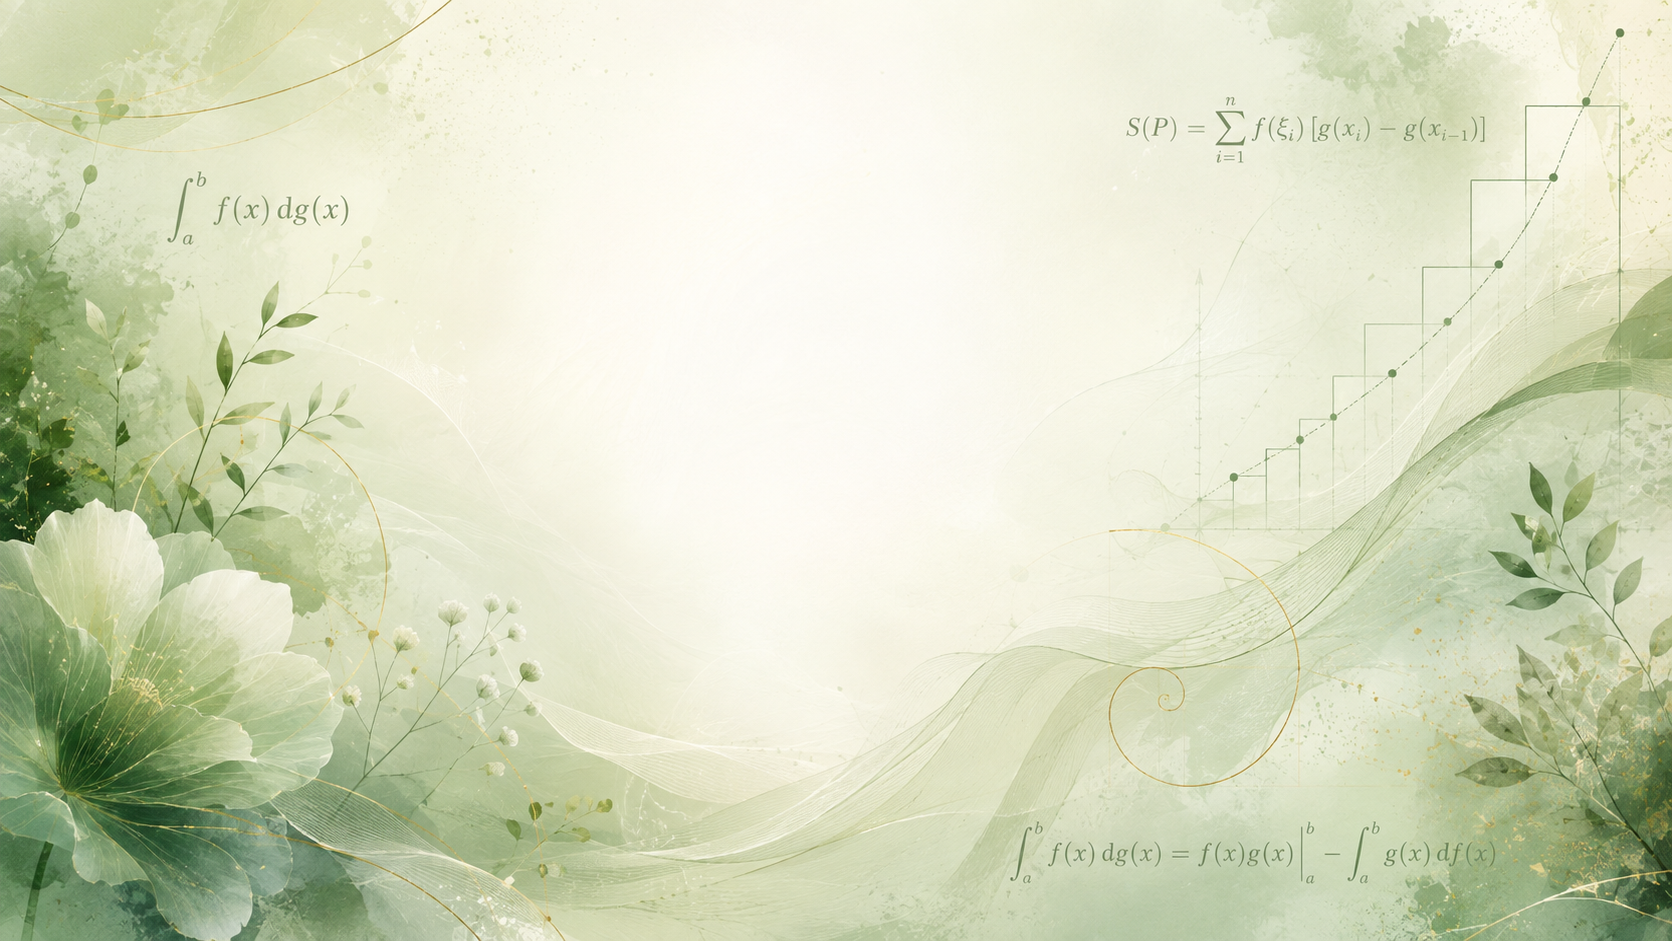
\includegraphics[width=\paperwidth,height=\paperheight,keepaspectratio=false]{chapter_06_bg_00.png}%
}
\begin{frame}[plain]
  \titlepage

  \note{
    Welcome to Chapter 6, Section 5: Rectifiable Curves. This is the
    final section of the chapter, and it is a reward for the work we
    have done so far: a topic of pure geometric interest that uses the
    integration theory we have built. The question is simple to state.
    What is the length of a curve? We will define a curve as a
    continuous mapping of an interval into "k" dimensional space,
    define its length as the supremum of the lengths of inscribed
    polygons, and then prove the formula that everyone remembers from
    calculus: for a continuously differentiable curve, the length is
    the integral of the speed. The proof combines the vector valued
    Fundamental Theorem and the triangle inequality for integrals from
    the previous section with uniform continuity. Let's begin.
  }
\end{frame}
}

{
\usebackgroundtemplate{%
  
\includegraphics[width=\paperwidth,height=\paperheight,keepaspectratio=false]{chapter_06_bg_01.png}%
}
\begin{frame}[c]{Outline}
  \begin{center}
    \tableofcontents
  \end{center}

  \note{
    Here is the plan for this episode. We start with some motivation:
    why the length of a curve is a natural question, and why the
    machinery of the previous section is exactly what is needed to
    answer it. Then we meet Definition 6.26, which says precisely what
    a curve is, and distinguishes arcs and closed curves. Next we
    define the length of a curve using inscribed polygons, and say
    what it means for a curve to be rectifiable. The heart of the
    episode is Theorem 6.27: for a continuously differentiable curve,
    the length equals the integral of the absolute value of the
    derivative. We prove it in two halves, one inequality in each
    direction. We close with a summary and a preview of Chapter 7.
  }
\end{frame}
\section{Motivation}

% --- Build 1/3 ---
\begin{frame}{Why This Section Matters}
  \begin{hlbox}
  \begin{itemize}
    \item A topic of \alert{geometric interest}: what is the
      \emph{length} of a curve in $R^k$?
  \end{itemize}
  \end{hlbox}

  \note{
    We begin with a question that sounds elementary. What is the
    length of a curve in "k" dimensional space? For a straight segment
    the answer is the distance between its endpoints. For a circle we
    learned a formula in school. But for a general curved path, what
    does length even mean? We have never defined it. Rudin ends this
    chapter with a topic of geometric interest, and the first job is
    to give the word length a precise meaning that does not depend on
    any formula.
  }
\end{frame}

% --- Build 2/3 ---
\begin{frame}{Why This Section Matters}
  \begin{hlbox}
  \begin{itemize}
    \item A topic of \alert{geometric interest}: what is the
      \emph{length} of a curve in $R^k$?
    \item An \alert{application} of the preceding theory: the vector
      integral results of Section 4 do the real work
  \end{itemize}
  \end{hlbox}

  \note{
    The second point is that this is an application of the theory we
    have just built. In the previous section we learned to integrate
    vector valued functions, we proved the Fundamental Theorem of
    Calculus for them, and we proved that the length of an integral is
    at most the integral of the length. Those two results, Theorem
    6.24 and Theorem 6.25, do the real work in today's main proof.
    So this section is not only about geometry; it shows the vector
    integral earning its keep.
  }
\end{frame}

% --- Build 3/3 ---
\begin{frame}{Why This Section Matters}
  \begin{hlbox}
  \begin{itemize}
    \item A topic of \alert{geometric interest}: what is the
      \emph{length} of a curve in $R^k$?
    \item An \alert{application} of the preceding theory: the vector
      integral results of Section 4 do the real work
    \item The case $k = 2$ (\emph{plane curves}) is central to
      \alert{complex analysis}
  \end{itemize}
  \end{hlbox}

  \note{
    Third, the special case "k" equals 2, that is, curves in the
    plane, is of considerable importance in the study of analytic
    functions of a complex variable. Complex analysis is built on
    integrals along curves in the complex plane, and a rectifiable
    curve is exactly the kind of path along which such integrals make
    sense. So although the setting today is general "k" dimensional
    space, keep the picture of a curve drawn in the plane in mind.
    Let's look at that picture now.
  }
\end{frame}

\begin{frame}{The Picture to Keep in Mind}
  \begin{center}
  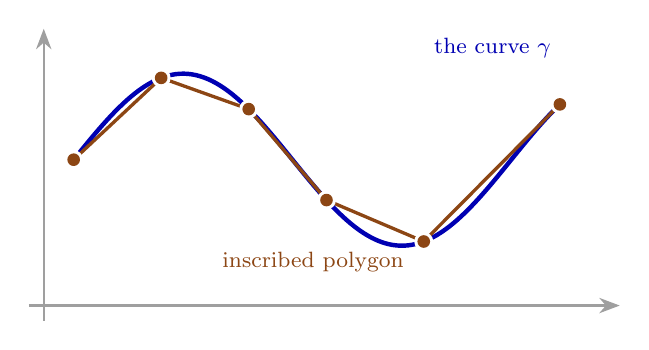
\begin{tikzpicture}[scale=0.95]
    \draw[axisln] (-0.6,-0.4) -- (7.3,-0.4);
    \draw[axisln] (-0.4,-0.6) -- (-0.4,3.3);
    % the curve
    \draw[curveln, blue!70!black]
      plot[domain=0:1, samples=120] ({\gx{\x}},{\gy{\x}});
    \node[blue!70!black] at (5.6,3.05) {\footnotesize the curve $\gamma$};
    % inscribed polygon
    \draw[chord, mAccent]
      ({\gx{0}},{\gy{0}}) -- ({\gx{0.18}},{\gy{0.18}}) -- ({\gx{0.36}},{\gy{0.36}})
      -- ({\gx{0.52}},{\gy{0.52}}) -- ({\gx{0.72}},{\gy{0.72}}) -- ({\gx{1}},{\gy{1}});
    \foreach \t in {0,0.18,0.36,0.52,0.72,1} {
      \dotpt{mAccent}{({\gx{\t}},{\gy{\t}})}
    }
    \node[mAccent, below] at (3.2,0.45) {\footnotesize inscribed polygon};
  \end{tikzpicture}
  \end{center}

  \vspace{-0.4em}
  \begin{center}
    \hl{\textbf{Length of $\gamma$} $=$ supremum of the lengths of all
    \textbf{inscribed polygons}}
  \end{center}

  \note{
    Here is the picture that organizes the whole section. The blue
    curve is a curve gamma in the plane, running from the left to the
    right. The orange dots are a handful of points on the curve, and
    the orange segments joining consecutive dots form an inscribed
    polygon. The length of a polygon is something we can compute: it
    is just a sum of distances between consecutive vertices. Notice
    that the polygon is shorter than the curve, because each orange
    segment is a straight shortcut between two points of the curve. As
    we add more and more vertices, the polygon hugs the curve more and
    more closely, and its length increases toward the length of the
    curve. That suggests the definition written under the picture: the
    length of gamma is the supremum of the lengths of all inscribed
    polygons. This is the definition we will adopt.
  }
\end{frame}

% --- Build 1/2 ---
\begin{frame}{What We Will Prove}
  \begin{hlbox}
  \begin{itemize}
    \item \textbf{Definition 6.26:} a \emph{curve} is a continuous map
      $\gamma : [a, b] \to R^k$; \emph{arcs}, \emph{closed curves};
      \\[2pt] \hspace{1.2em} length
      $\Lambda(\gamma) = \sup_P \Lambda(P, \gamma)$;
      \emph{rectifiable} if $\Lambda(\gamma) < \infty$
  \end{itemize}
  \end{hlbox}

  \note{
    Let's preview the two items of this section. First, Definition
    6.26. A curve is a continuous mapping gamma from a closed interval
    "a" "b" into "k" dimensional space. A one to one curve is called an
    arc, and a curve whose two endpoints coincide is called a closed
    curve. The same definition introduces the length of a curve as
    the supremum over all partitions capital "P" of the lengths of the
    inscribed polygons, and calls a curve rectifiable when this
    supremum is finite.
  }
\end{frame}

% --- Build 2/2 ---
\begin{frame}{What We Will Prove}
  \begin{hlbox}
  \begin{itemize}
    \item \textbf{Definition 6.26:} a \emph{curve} is a continuous map
      $\gamma : [a, b] \to R^k$; \emph{arcs}, \emph{closed curves};
      \\[2pt] \hspace{1.2em} length
      $\Lambda(\gamma) = \sup_P \Lambda(P, \gamma)$;
      \emph{rectifiable} if $\Lambda(\gamma) < \infty$
    \item \textbf{Theorem 6.27:} if $\gamma'$ is continuous on $[a, b]$,
      then $\gamma$ is rectifiable and
      \[
        \Lambda(\gamma) = \int_a^b |\gamma'(t)|\,dt
      \]
      \hspace{1.2em} \emph{length equals the integral of the speed}
  \end{itemize}
  \end{hlbox}

  \note{
    Second, Theorem 6.27, the main result. If the derivative of gamma
    exists and is continuous on the whole interval, then gamma is
    rectifiable, and its length is given by a Riemann integral: the
    integral from "a" to "b" of the absolute value of gamma prime of
    "t". If you think of gamma of "t" as the position of a moving
    point at time "t", then gamma prime is its velocity and the
    absolute value of gamma prime is its speed. The theorem says that
    the distance traveled is the integral of the speed, which is
    exactly what physical intuition predicts. Let's start with the
    definitions.
  }
\end{frame}
}

{
\usebackgroundtemplate{%
  
\includegraphics[width=\paperwidth,height=\paperheight,keepaspectratio=false]{chapter_06_bg_02.png}%
}
\section{Curves in $R^k$}

% --- Build 1/3 ---
\begin{frame}{Definition 6.26: Curves, Arcs, Closed Curves}
  \begin{defblock}{Definition 6.26}
    A \alert{continuous} mapping $\gamma$ of an interval $[a, b]$ into
    $R^k$ is called a \alert{curve} in $R^k$. To emphasize the parameter
    interval $[a, b]$, we may also say that $\gamma$ is a curve
    \emph{on} $[a, b]$.
  \end{defblock}

  \note{
    Here is the first part of Definition 6.26. A curve in "k"
    dimensional space is a continuous mapping gamma from a closed
    interval "a" "b" into that space. Continuity is the only
    requirement: the mapping need not be differentiable, and it need
    not be one to one, so the curve may cross itself. The variable
    "t" in the interval is called the parameter, and it is often
    useful to think of it as time, so that gamma of "t" is the
    position of a moving point at time "t". When we want to emphasize
    the parameter interval, we say that gamma is a curve on the
    interval "a" "b". Next, two special kinds of curves.
  }
\end{frame}

% --- Build 2/3 ---
\begin{frame}{Definition 6.26: Curves, Arcs, Closed Curves}
  \begin{defblock}{Definition 6.26}
    A \alert{continuous} mapping $\gamma$ of an interval $[a, b]$ into
    $R^k$ is called a \alert{curve} in $R^k$. To emphasize the parameter
    interval $[a, b]$, we may also say that $\gamma$ is a curve
    \emph{on} $[a, b]$.

    \vspace{0.3em}
    If $\gamma$ is \emph{one-to-one}, $\gamma$ is called an \alert{arc}.
  \end{defblock}

  \note{
    If gamma is one to one, meaning that distinct parameter values are
    sent to distinct points, then gamma is called an arc. An arc never
    crosses itself and never retraces its steps. In particular, since
    "a" and "b" are different parameter values, an arc has two
    different endpoints.
  }
\end{frame}

% --- Build 3/3 ---
\begin{frame}{Definition 6.26: Curves, Arcs, Closed Curves}
  \begin{defblock}{Definition 6.26}
    A \alert{continuous} mapping $\gamma$ of an interval $[a, b]$ into
    $R^k$ is called a \alert{curve} in $R^k$. To emphasize the parameter
    interval $[a, b]$, we may also say that $\gamma$ is a curve
    \emph{on} $[a, b]$.

    \vspace{0.3em}
    If $\gamma$ is \emph{one-to-one}, $\gamma$ is called an \alert{arc}.

    \vspace{0.3em}
    If $\gamma(a) = \gamma(b)$, $\gamma$ is said to be a
    \alert{closed curve}.
  \end{defblock}

  \note{
    If gamma of "a" equals gamma of "b", that is, if the moving point
    ends exactly where it started, gamma is said to be a closed curve.
    A circle traversed once is the standard example. Notice that a
    closed curve is never an arc, because the two endpoints of the
    parameter interval are sent to the same point. Let's look at
    pictures of these three situations.
  }
\end{frame}

\begin{frame}{Three Kinds of Curves}
  \begin{center}
  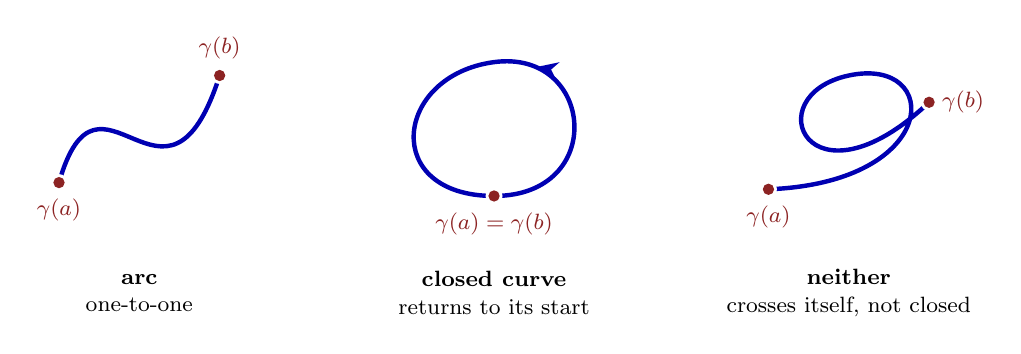
\begin{tikzpicture}[scale=0.85]
    % --- arc ---
    \begin{scope}[shift={(0,0)}]
      \draw[curveln, blue!70!black]
        (0,0.3) .. controls (0.6,2.4) and (1.6,-0.6) .. (2.4,1.9);
      \dotpt{thmcolor}{(0,0.3)}
      \dotpt{thmcolor}{(2.4,1.9)}
      \node[thmcolor, below] at (0,0.2) {\footnotesize $\gamma(a)$};
      \node[thmcolor, above] at (2.4,2.0) {\footnotesize $\gamma(b)$};
      \node[align=center] at (1.2,-1.35) {\footnotesize \textbf{arc}\\[-2pt]
        \footnotesize one-to-one};
    \end{scope}
    % --- closed curve ---
    \begin{scope}[shift={(5.3,0)}]
      \draw[curveln, blue!70!black]
        (1.2,0.1) .. controls (2.9,0.1) and (2.7,2.3) .. (1.2,2.1)
        .. controls (-0.3,1.9) and (-0.5,0.1) .. (1.2,0.1);
      \draw[guide, blue!70!black] (1.9,2.02) -- (1.85,2.03);
      \dotpt{thmcolor}{(1.2,0.1)}
      \node[thmcolor, below] at (1.2,0.0) {\footnotesize $\gamma(a) = \gamma(b)$};
      \node[align=center] at (1.2,-1.35) {\footnotesize \textbf{closed curve}\\[-2pt]
        \footnotesize returns to its start};
    \end{scope}
    % --- neither ---
    \begin{scope}[shift={(10.6,0)}]
      \draw[curveln, blue!70!black]
        (0,0.2) .. controls (2.6,0.3) and (2.6,2.2) .. (1.2,1.9)
        .. controls (-0.2,1.6) and (0.6,-0.2) .. (2.4,1.5);
      \dotpt{thmcolor}{(0,0.2)}
      \dotpt{thmcolor}{(2.4,1.5)}
      \node[thmcolor, below] at (0,0.1) {\footnotesize $\gamma(a)$};
      \node[thmcolor, right] at (2.45,1.5) {\footnotesize $\gamma(b)$};
      \node[align=center] at (1.2,-1.35) {\footnotesize \textbf{neither}\\[-2pt]
        \footnotesize crosses itself, not closed};
    \end{scope}
  \end{tikzpicture}
  \end{center}

  \vspace{0.2em}
  \begin{center}
    \hl{All three are \emph{curves}: continuous maps $\gamma : [a, b] \to R^k$.}
  \end{center}

  \note{
    Here are three curves, drawn in blue, with their endpoints marked
    in red. On the left is an arc: the moving point starts at gamma of
    "a", wanders through a bend, and ends at a different point gamma
    of "b" without ever crossing its own path. In the middle is a
    closed curve: a loop in which the start and the end are the same
    point, labeled gamma of "a" equals gamma of "b"; the small arrow
    shows the direction of travel. On the right is a curve that is
    neither: it crosses itself, so it is not one to one and hence not
    an arc, and its endpoints gamma of "a" and gamma of "b" are
    different, so it is not closed. The sentence under the picture
    makes the main point: all three are perfectly good curves, since
    the only requirement in the definition is continuity. Next, an
    important subtlety about what a curve really is.
  }
\end{frame}

% --- Build 1/2 ---
\begin{frame}{A Curve Is a Mapping, Not a Point Set}
  \begin{remblock}{Remark}
    A curve is defined to be a \alert{mapping}, not a point set.
    Each curve $\gamma$ has an associated subset of $R^k$, its
    \emph{range} $\gamma([a, b])$, but \alert{different curves may have
    the same range}.
  \end{remblock}

  \note{
    Rudin makes a point of this remark, and it deserves a slide of its
    own. A curve is the mapping gamma, not the set of points it traces
    out. Of course every curve has a range, the set of all values
    gamma of "t", and this range is the geometric object we would draw
    on paper. But the same set of points can be traced out in many
    different ways: at different speeds, in different directions, or
    several times over. Different mappings mean different curves, even
    when the drawings look identical. Let's see the standard example.
  }
\end{frame}

% --- Build 2/2 ---
\begin{frame}{A Curve Is a Mapping, Not a Point Set}
  \begin{remblock}{Remark}
    A curve is defined to be a \alert{mapping}, not a point set.
    Each curve $\gamma$ has an associated subset of $R^k$, its
    \emph{range} $\gamma([a, b])$, but \alert{different curves may have
    the same range}.
  \end{remblock}

  \begin{exblock}{Example: same range, different curves}
    \vspace{0.3em}
    \begin{minipage}{0.48\linewidth}
      \centering
      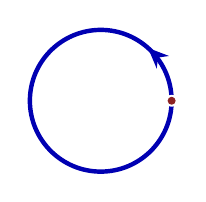
\begin{tikzpicture}[scale=0.6]
        \draw[curveln, blue!70!black] (0,0) circle (1.5);
        \draw[guide, blue!70!black] (1.06,1.06) -- (1.0,1.118);
        \dotpt{thmcolor}{(1.5,0)}
      \end{tikzpicture}\\[2pt]
      {\footnotesize $\gamma_1(t) = (\cos t, \sin t)$, $0 \leq t \leq 2\pi$}
    \end{minipage}\hfill
    \begin{minipage}{0.48\linewidth}
      \centering
      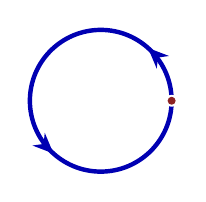
\begin{tikzpicture}[scale=0.6]
        \draw[curveln, blue!70!black] (0,0) circle (1.5);
        \draw[guide, blue!70!black] (1.06,1.06) -- (1.0,1.118);
        \draw[guide, blue!70!black] (-1.06,-1.06) -- (-1.0,-1.118);
        \dotpt{thmcolor}{(1.5,0)}
      \end{tikzpicture}\\[2pt]
      {\footnotesize $\gamma_2(t) = (\cos 2t, \sin 2t)$, $0 \leq t \leq 2\pi$}
    \end{minipage}
  \end{exblock}

  \note{
    On the left, gamma sub 1 sends "t" to the point with coordinates
    cosine "t" and sine "t", for "t" between 0 and 2 pi. Its range is
    the unit circle, traversed once counterclockwise, starting and
    ending at the red point. On the right, gamma sub 2 sends "t" to
    cosine of 2 "t" and sine of 2 "t", on the same parameter interval.
    The range is again the unit circle, but the point now moves twice
    as fast and goes around twice, as the two arrows suggest. The two
    drawings are indistinguishable, yet gamma sub 1 and gamma sub 2
    are different mappings, hence different curves. We will see
    shortly that they even have different lengths: 2 pi and 4 pi.
    Length is a property of the mapping, not of the range. Now let's
    define length.
  }
\end{frame}
}

{
\usebackgroundtemplate{%
  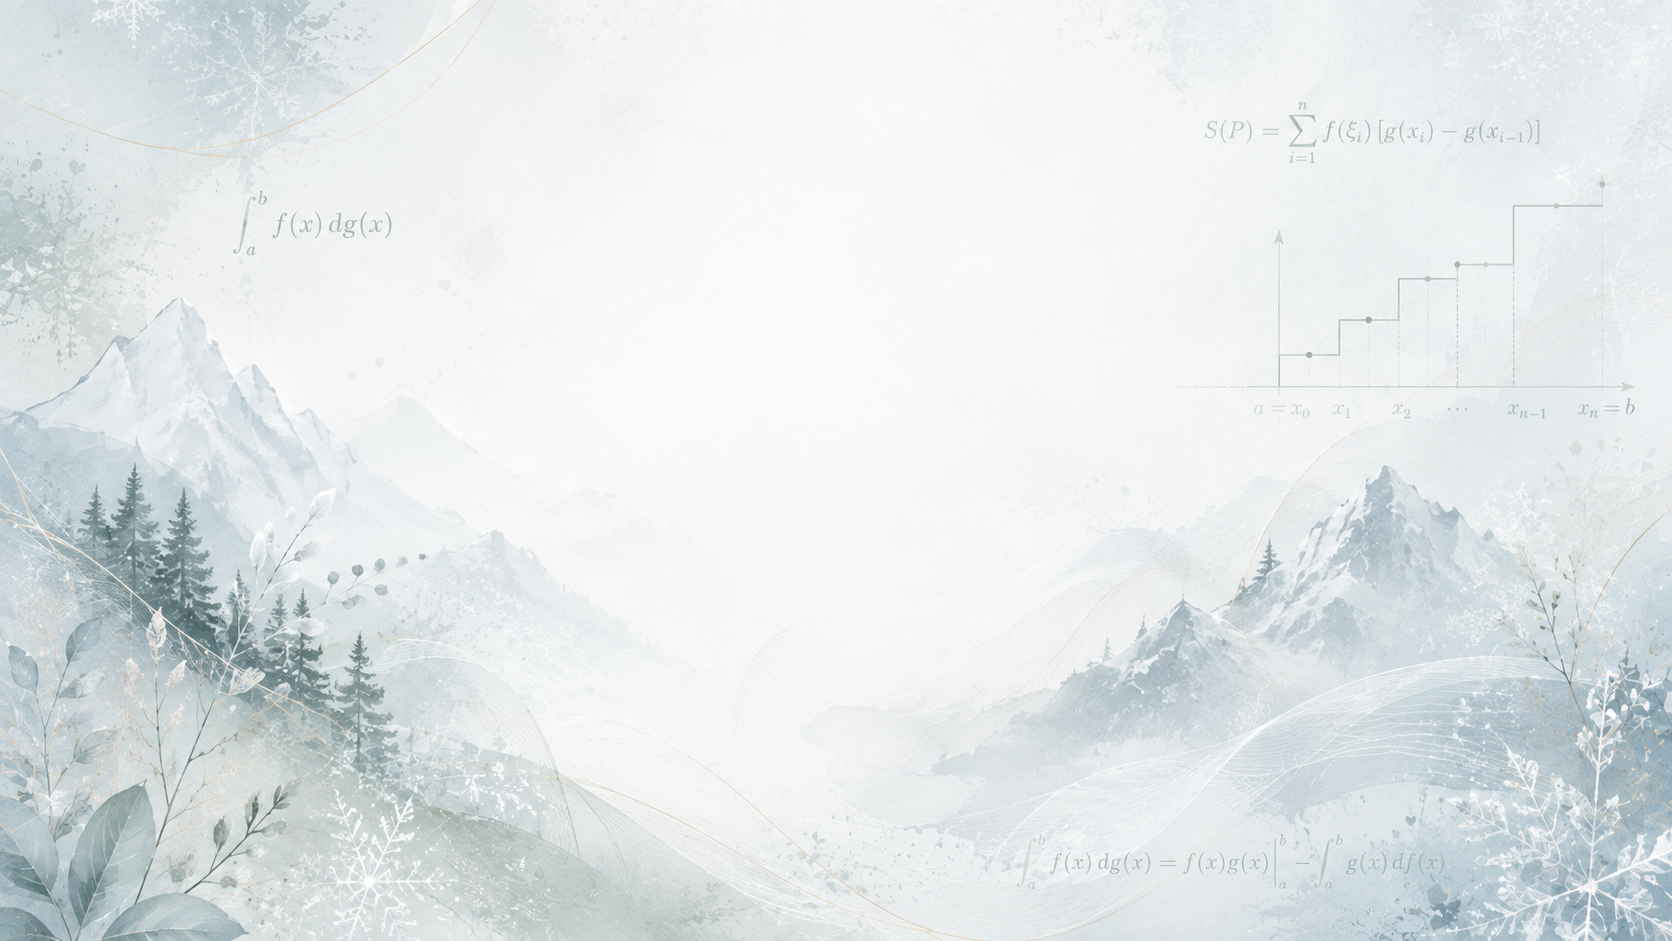
\includegraphics[width=\paperwidth,height=\paperheight,keepaspectratio=false]{chapter_06_bg_03.png}%
}
\section{The Length of a Curve}

% --- Build 1/2 ---
\begin{frame}{Inscribed Polygons}
  \begin{defblock}{Definition 6.26 (continued): the polygonal length}
    To each partition $P = \{x_0, \dots, x_n\}$ of $[a, b]$ and each curve
    $\gamma$ on $[a, b]$ we associate the number
    \[
      \Lambda(P, \gamma) = \sum_{i=1}^{n} |\gamma(x_i) - \gamma(x_{i-1})|.
    \]
  \end{defblock}

  \note{
    Now we make the picture from the beginning of the episode precise.
    Take any partition capital "P" of the parameter interval, with
    points "x" sub 0 up to "x" sub "n", and take any curve gamma on
    that interval. To this pair we associate the number Lambda of
    capital "P" and gamma, defined by the sum on the slide. The term
    with index "i" is the absolute value of gamma of "x" sub "i" minus
    gamma of "x" sub "i" minus 1. Remember that absolute value in "k"
    dimensional space means Euclidean length, so this term is the
    distance between two consecutive points on the curve. Let's draw
    it.
  }
\end{frame}

% --- Build 2/2 ---
\begin{frame}{Inscribed Polygons}
  \begin{defblock}{Definition 6.26 (continued): the polygonal length}
    To each partition $P = \{x_0, \dots, x_n\}$ of $[a, b]$ and each curve
    $\gamma$ on $[a, b]$ we associate the number
    \[
      \Lambda(P, \gamma) = \sum_{i=1}^{n} |\gamma(x_i) - \gamma(x_{i-1})|.
    \]
  \end{defblock}

  \vspace{-0.5em}
  \begin{center}
  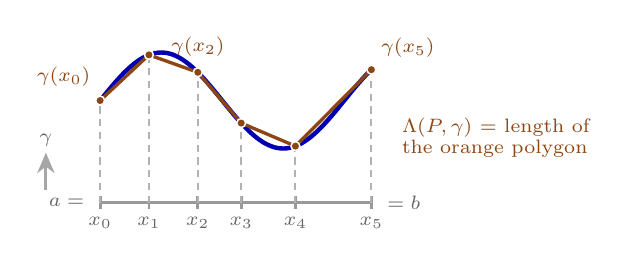
\begin{tikzpicture}[scale=0.53]
    % parameter interval
    \draw[line width=1pt, gray!80] ({\gx{0}},-0.9) -- ({\gx{1}},-0.9);
    \foreach \t/\lab in {0/x_0, 0.18/x_1, 0.36/x_2, 0.52/x_3, 0.72/x_4, 1/x_5} {
      \draw[gray!80, line width=1pt] ({\gx{\t}},-1.05) -- ({\gx{\t}},-0.75);
      \node[gray!80!black, below] at ({\gx{\t}},-1.02) {\scriptsize $\lab$};
      \draw[projln, gray!60] ({\gx{\t}},-0.9) -- ({\gx{\t}},{\gy{\t}});
    }
    \node[gray!80!black, left] at ({\gx{0}-0.15},-0.9) {\scriptsize $a =$};
    \node[gray!80!black, right] at ({\gx{1}+0.15},-0.9) {\scriptsize $= b$};
    \node[gray!80!black] at (-1.3,0.6) {\scriptsize $\gamma$};
    \draw[guide, gray!70] (-1.3,-0.6) -- (-1.3,0.3);
    % the curve
    \draw[curveln, blue!70!black]
      plot[domain=0:1, samples=120] ({\gx{\x}},{\gy{\x}});
    % polygon
    \draw[chord, mAccent]
      ({\gx{0}},{\gy{0}}) -- ({\gx{0.18}},{\gy{0.18}}) -- ({\gx{0.36}},{\gy{0.36}})
      -- ({\gx{0.52}},{\gy{0.52}}) -- ({\gx{0.72}},{\gy{0.72}}) -- ({\gx{1}},{\gy{1}});
    \foreach \t in {0,0.18,0.36,0.52,0.72,1} {
      \dotpt{mAccent}{({\gx{\t}},{\gy{\t}})}
    }
    \node[mAccent, above left] at ({\gx{0}},{\gy{0}+0.1}) {\scriptsize $\gamma(x_0)$};
    \node[mAccent, above] at ({\gx{0.36}},{\gy{0.36}+0.15}) {\scriptsize $\gamma(x_2)$};
    \node[mAccent, above right] at ({\gx{1}},{\gy{1}+0.05}) {\scriptsize $\gamma(x_5)$};
    \node[mAccent, right] at (7.0,0.9) {\scriptsize $\Lambda(P, \gamma)$ = length of};
    \node[mAccent, right] at (7.0,0.4) {\scriptsize the orange polygon};
  \end{tikzpicture}
  \end{center}

  \note{
    In the picture, the gray line at the bottom is the parameter
    interval from "a" to "b", with the partition points "x" sub 0
    through "x" sub 5 marked by ticks. The map gamma, indicated by the
    gray arrow on the left, sends each partition point up along a
    dashed line to a point on the blue curve; three of these image
    points are labeled gamma of "x" sub 0, gamma of "x" sub 2, and
    gamma of "x" sub 5. Joining consecutive image points by straight
    segments gives the orange polygon. Each orange segment has length
    equal to one term of the sum, so Lambda of capital "P" and gamma
    is the total length of the orange polygon, whose vertices are the
    points gamma of "x" sub 0 through gamma of "x" sub "n", in this
    order. Next, what happens when we refine the partition.
  }
\end{frame}

\begin{frame}{Refining the Partition}
  \begin{center}
  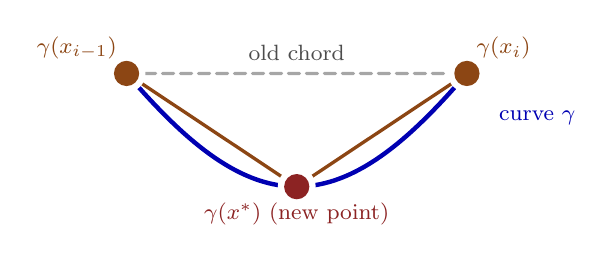
\begin{tikzpicture}[scale=1.9]
    \draw[curveln, blue!70!black]
      plot[domain=0.50:0.85, samples=80] ({\gx{\x}},{\gy{\x}});
    % old chord
    \draw[chord, gray!70, dash pattern=on 4pt off 2.5pt]
      ({\gx{0.50}},{\gy{0.50}}) -- ({\gx{0.85}},{\gy{0.85}});
    % new chords
    \draw[chord, mAccent]
      ({\gx{0.50}},{\gy{0.50}}) -- ({\gx{0.675}},{\gy{0.675}}) -- ({\gx{0.85}},{\gy{0.85}});
    \dotpt{mAccent}{({\gx{0.50}},{\gy{0.50}})}
    \dotpt{mAccent}{({\gx{0.85}},{\gy{0.85}})}
    \dotpt{thmcolor}{({\gx{0.675}},{\gy{0.675}})}
    \node[mAccent, above left] at ({\gx{0.50}},{\gy{0.50}+0.03}) {\footnotesize $\gamma(x_{i-1})$};
    \node[mAccent, above right] at ({\gx{0.85}},{\gy{0.85}+0.03}) {\footnotesize $\gamma(x_i)$};
    \node[thmcolor, below] at ({\gx{0.675}},{\gy{0.675}-0.04}) {\footnotesize $\gamma(x^*)$ (new point)};
    \node[gray!60!black, above] at ({\gx{0.675}},{\gy{0.50}+0.02}) {\footnotesize old chord};
    \node[blue!70!black, right] at ({\gx{0.85}+0.15},{\gy{0.85}-0.3}) {\footnotesize curve $\gamma$};
  \end{tikzpicture}
  \end{center}

  \vspace{-0.3em}
  \begin{hlbox}
  \begin{center}
    Triangle inequality:
    $|\gamma(x_i) - \gamma(x_{i-1})| \leq |\gamma(x^*) - \gamma(x_{i-1})| + |\gamma(x_i) - \gamma(x^*)|$
    \\[3pt]
    so $P^* \supset P \;\Longrightarrow\; \Lambda(P^*, \gamma) \geq \Lambda(P, \gamma)$:
    \alert{refining never shortens the polygon}
  \end{center}
  \end{hlbox}

  \note{
    Here is a useful observation that is not stated in the book but
    explains why the definition of length is the right one. The blue
    arc is one piece of the curve, between the two orange vertices
    gamma of "x" sub "i" minus 1 and gamma of "x" sub "i". The dashed
    gray segment is the old chord joining them. Now insert a new
    partition point "x" star between "x" sub "i" minus 1 and "x" sub
    "i"; its image is the red dot. The old chord is replaced by the two
    orange chords through the red dot. By the triangle inequality,
    written under the picture, the two new chords together are at
    least as long as the old chord. So refining a partition can only
    increase the polygonal length, never decrease it. As partitions
    get finer, the polygon approaches the curve more and more closely,
    and its length creeps upward. This is why the supremum over all
    partitions is the natural definition of length.
  }
\end{frame}

% --- Build 1/2 ---
\begin{frame}{Definition 6.26: Length and Rectifiability}
  \begin{defblock}{Definition 6.26 (continued): the length of a curve}
    The \alert{length} of $\gamma$ is
    \[
      \Lambda(\gamma) = \sup_{P} \Lambda(P, \gamma),
    \]
    where the supremum is taken over \emph{all} partitions $P$ of $[a, b]$.
  \end{defblock}

  \note{
    We are now ready for the definition. The length of gamma, written
    Lambda of gamma, is the supremum of Lambda of capital "P" and
    gamma over all partitions capital "P" of the interval "a" "b". In
    words, the length of a curve is the least upper bound of the
    lengths of all inscribed polygons. Because every polygonal length
    is a nonnegative real number, this supremum always exists in the
    extended real number system; it is either a nonnegative real
    number or plus infinity. Note that no derivative is involved. The
    definition uses only continuity and distances, so it applies to
    every curve.
  }
\end{frame}

% --- Build 2/2 ---
\begin{frame}{Definition 6.26: Length and Rectifiability}
  \begin{defblock}{Definition 6.26 (continued): the length of a curve}
    The \alert{length} of $\gamma$ is
    \[
      \Lambda(\gamma) = \sup_{P} \Lambda(P, \gamma),
    \]
    where the supremum is taken over \emph{all} partitions $P$ of $[a, b]$.

    \vspace{0.3em}
    If $\Lambda(\gamma) < \infty$, we say that $\gamma$ is \alert{rectifiable}.
  \end{defblock}

  \vspace{0.3em}
  \begin{hlbox}
  \textbf{Note:} $\Lambda(\gamma)$ always exists in $[0, +\infty]$;\\
  \emph{rectifiable} means the curve has \emph{finite} length.
  \end{hlbox}

  \note{
    If the length Lambda of gamma is finite, we say that gamma is
    rectifiable. The word comes from the Latin for straightening: a
    rectifiable curve is one that could, in principle, be straightened
    out into a segment of finite length. As the note on the slide
    says, the length itself is always defined, possibly as plus
    infinity; rectifiability is the statement that it is finite. You
    might wonder whether a continuous curve can really have infinite
    length. It can, and the next slide shows the classic example.
  }
\end{frame}

\begin{frame}{Not Every Curve Is Rectifiable}
  \begin{columns}[T]
    \begin{column}{0.5\textwidth}
      \begin{center}
      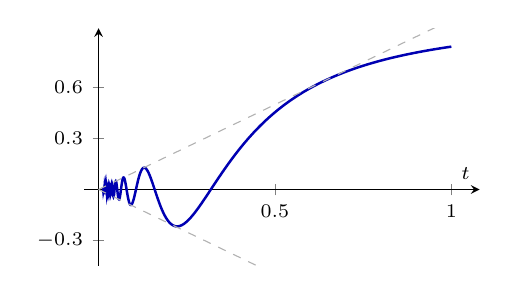
\begin{tikzpicture}
        \begin{axis}[
          width=6.6cm, height=4.6cm,
          axis lines=middle,
          xmin=-0.04, xmax=1.08, ymin=-0.45, ymax=0.95,
          xtick={0.5,1}, ytick={-0.3,0.3,0.6},
          ticklabel style={font=\scriptsize},
          xlabel={\scriptsize $t$}, ylabel={},
        ]
          \addplot[blue!70!black, line width=0.9pt, domain=0.012:1, samples=1200, smooth]
            {x*sin(deg(1/x))};
          \addplot[gray!60, dashed, domain=0:1, samples=2] {x};
          \addplot[gray!60, dashed, domain=0:1, samples=2] {-x};
        \end{axis}
      \end{tikzpicture}
      \end{center}
    \end{column}
    \begin{column}{0.48\textwidth}
      \begin{remblock}{Example}
        $\gamma(t) = \big(t,\, t \sin(1/t)\big)$ for $0 < t \leq 1$,
        $\gamma(0) = (0, 0)$.

        \vspace{0.3em}
        $\gamma$ is a \emph{continuous} curve in $R^2$, but
        $\Lambda(\gamma) = +\infty$: it is \alert{not rectifiable}.
      \end{remblock}

      \vspace{0.2em}
      \begin{hlbox}
      {\footnotesize \textbf{Why:} the oscillations near $t = 0$ have heights
      $\approx \tfrac{2}{(2m+1)\pi}$, and $\sum \tfrac{1}{m}$ diverges.}
      \end{hlbox}
    \end{column}
  \end{columns}

  \note{
    On the left is the graph of "t" times sine of 1 over "t", between
    the dashed lines "y" equals "t" and "y" equals minus "t". The
    corresponding curve gamma, defined in the gray box, sends "t" to
    the point "t" comma "t" sine of 1 over "t", with gamma of 0 equal
    to the origin. This curve is continuous, even at 0, because the
    factor "t" squeezes the oscillation to zero. But look at how
    wildly it oscillates as "t" approaches 0. Number the oscillations
    from the right by "m". Oscillation number "m" is a little up and
    down of height roughly 2 over the quantity 2 "m" plus 1 times pi,
    so its height shrinks like 1 over "m". Inscribing a polygon that
    visits the tops and bottoms of the first few hundred oscillations
    gives a length at least a constant times 1 plus one half plus one
    third and so on, and that harmonic sum diverges. So the supremum of the
    polygonal lengths is infinite, and gamma is not rectifiable.
    Continuity alone does not guarantee finite length. Something more
    is needed, and that brings us to differentiable curves.
  }
\end{frame}

% --- Build 1/2 ---
\begin{frame}{When Is the Length an Integral?}
  \begin{hlbox}
  \begin{itemize}
    \item In certain cases $\Lambda(\gamma)$ is given by a
      \alert{Riemann integral}
    \item We prove this for \alert{continuously differentiable} curves:
      $\gamma'$ exists and is continuous on $[a, b]$
  \end{itemize}
  \end{hlbox}

  \note{
    The supremum definition is conceptually clean, but it is hopeless
    for computing. Fortunately, in certain cases the length is given
    by a Riemann integral, and that is the content of the main
    theorem. We prove it for continuously differentiable curves, that
    is, curves gamma whose derivative gamma prime exists at every point
    of the interval and is continuous there. Recall from Chapter 5,
    Section 7 that the derivative of a vector valued function is
    computed componentwise, and that gamma prime of "t" is the
    velocity vector of the moving point at time "t". What should the
    integral be?
  }
\end{frame}

% --- Build 2/2 ---
\begin{frame}{When Is the Length an Integral?}
  \begin{hlbox}
  \begin{itemize}
    \item In certain cases $\Lambda(\gamma)$ is given by a
      \alert{Riemann integral}
    \item We prove this for \alert{continuously differentiable} curves:
      $\gamma'$ exists and is continuous on $[a, b]$
    \item \textbf{Heuristic:} $\gamma'(t)$ = velocity, $|\gamma'(t)|$ = speed,
      so over a short time $\Delta x_i$:
      \begin{gather*}
        |\gamma(x_i) - \gamma(x_{i-1})| \approx |\gamma'(x_i)|\,\Delta x_i, \\
        \Lambda(P, \gamma) \approx \sum_i |\gamma'(x_i)|\,\Delta x_i
        \;\longrightarrow\; \int_a^b |\gamma'(t)|\,dt
      \end{gather*}
  \end{itemize}
  \end{hlbox}

  \note{
    Here is the heuristic. Over a very short time interval, whose
    width the slide calls delta "x" sub "i", a differentiable curve is
    almost a straight segment, and the velocity is almost constant. So the chord length,
    the distance between gamma of "x" sub "i" minus 1 and gamma of "x"
    sub "i", is approximately the speed at "x" sub "i" times the time
    elapsed. Adding these approximations over all subintervals turns
    the polygonal length into a Riemann sum for the function absolute
    value of gamma prime, and as the partition gets finer the Riemann
    sum tends to the integral of the speed. Making this heuristic
    rigorous is exactly what the proof of Theorem 6.27 does. Let's
    state the theorem.
  }
\end{frame}
}

{
\usebackgroundtemplate{%
  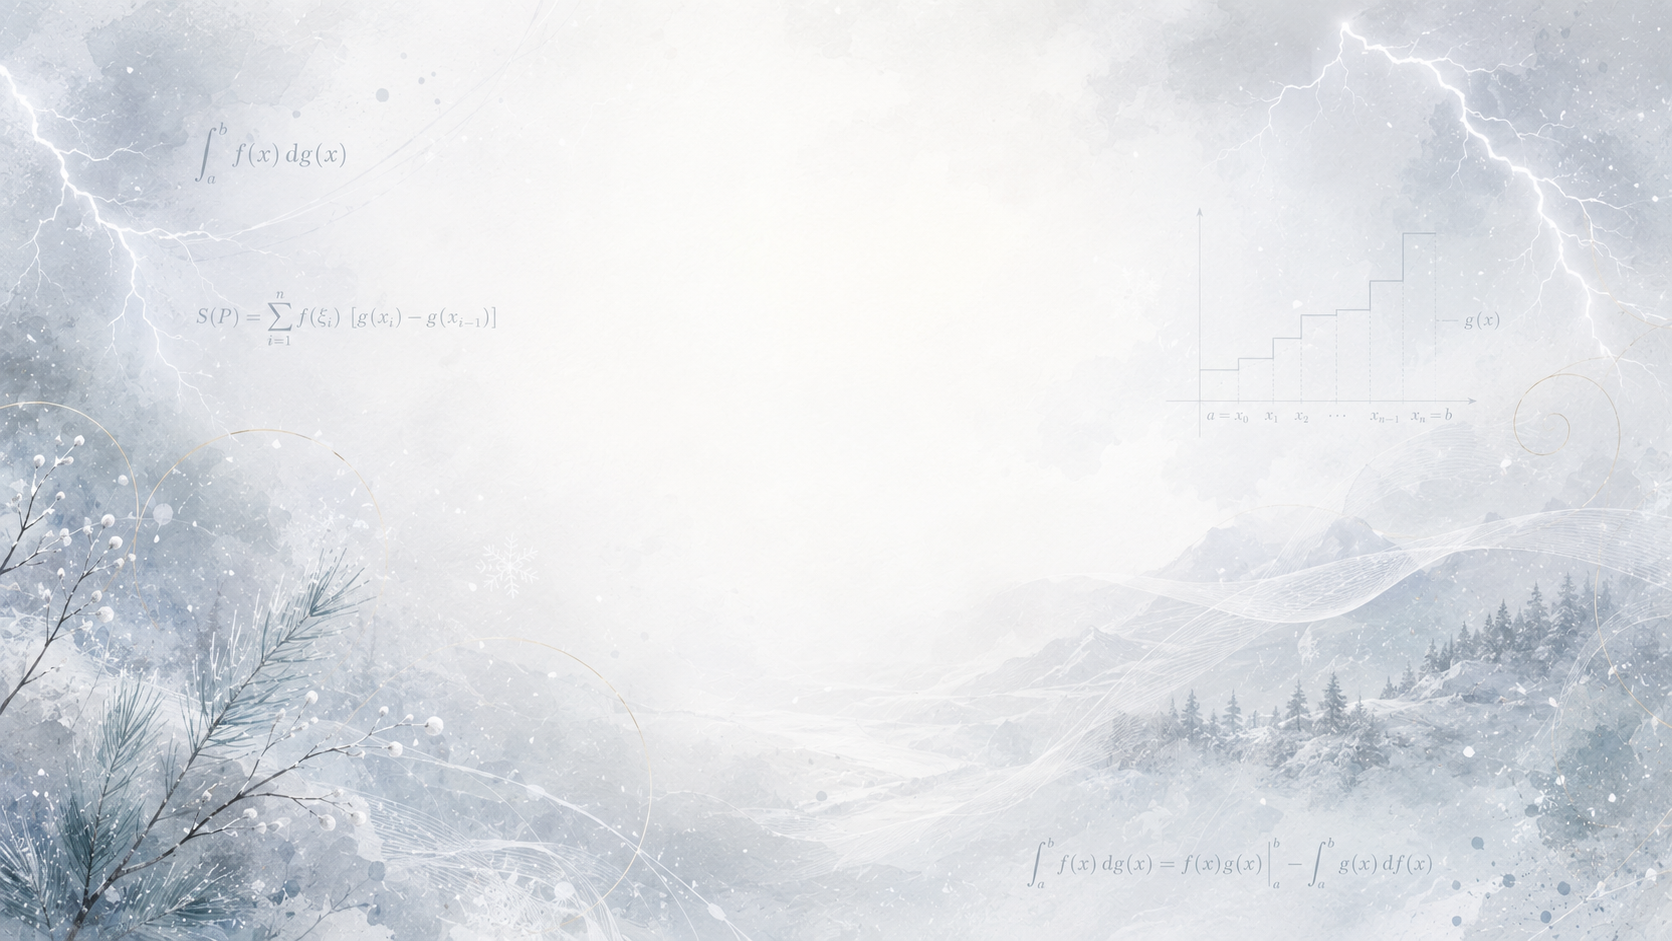
\includegraphics[width=\paperwidth,height=\paperheight,keepaspectratio=false]{chapter_06_bg_04.png}%
}
\section{Length as an Integral}

% --- Build 1/2 ---
\begin{frame}{Theorem 6.27: Length of a Continuously Differentiable Curve}
  \begin{thmblock}{Theorem 6.27}
    If $\gamma'$ is continuous on $[a, b]$, then $\gamma$ is rectifiable, and
    \[
      \Lambda(\gamma) = \int_a^b |\gamma'(t)|\,dt.
    \]
  \end{thmblock}

  \note{
    Theorem 6.27 says: if gamma prime is continuous on the closed
    interval "a" "b", then gamma is rectifiable, and its length is the
    integral from "a" to "b" of the absolute value of gamma prime of
    "t". Two things are being claimed. First, the length is finite.
    Second, it equals a specific integral. Notice that the integral
    makes sense: the integrand is the composition of the continuous
    vector function gamma prime with the continuous Euclidean norm, so
    it is a continuous real function on the interval, and continuous
    functions are Riemann integrable by Theorem 6.8.
  }
\end{frame}

% --- Build 2/2 ---
\begin{frame}{Theorem 6.27: Length of a Continuously Differentiable Curve}
  \begin{thmblock}{Theorem 6.27}
    If $\gamma'$ is continuous on $[a, b]$, then $\gamma$ is rectifiable, and
    \[
      \Lambda(\gamma) = \int_a^b |\gamma'(t)|\,dt.
    \]
  \end{thmblock}

  \vspace{0.3em}
  \begin{hlbox}
  \textbf{Key idea:} \alert{distance traveled $=$ integral of speed.}

  \vspace{0.4em}
  In coordinates, $\gamma = (\gamma_1, \dots, \gamma_k)$ and
  $\displaystyle \Lambda(\gamma) = \int_a^b \sqrt{\gamma_1'(t)^2 + \cdots + \gamma_k'(t)^2}\,dt$,
  the familiar \emph{arc length formula} from calculus.
  \end{hlbox}

  \note{
    The key idea is the physical one: distance traveled is the
    integral of speed. If we write gamma in coordinates, as a "k"
    tuple of real functions gamma sub 1 through gamma sub "k", then
    the absolute value of gamma prime is the square root of the sum of
    the squares of the coordinate derivatives, and the theorem becomes
    the arc length formula from calculus, displayed at the bottom of
    the slide. In a calculus course this formula is usually taken as
    the definition of arc length. Here it is a theorem: length was
    defined geometrically, via inscribed polygons, and the formula is
    proved from that definition. Before the proof, let's test the
    theorem on the circle.
  }
\end{frame}

% --- Build 1/2 ---
\begin{frame}{Example: The Unit Circle}
  \begin{columns}[T]
    \begin{column}{0.34\textwidth}
      \begin{center}
      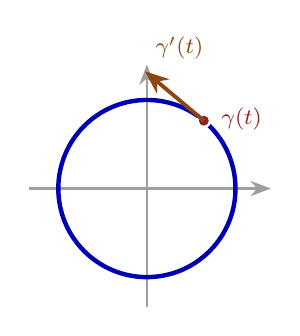
\begin{tikzpicture}[scale=0.75]
        \draw[axisln] (-2,0) -- (2.1,0);
        \draw[axisln] (0,-2) -- (0,2.1);
        \draw[curveln, blue!70!black] (0,0) circle (1.5);
        \dotpt{thmcolor}{({1.5*cos(50)},{1.5*sin(50)})}
        \draw[vec, mAccent] ({1.5*cos(50)},{1.5*sin(50)})
          -- ({1.5*cos(50)-1.3*sin(50)},{1.5*sin(50)+1.3*cos(50)});
        \node[mAccent, anchor=south] at (0.55,2.02) {\footnotesize $\gamma'(t)$};
        \node[thmcolor, anchor=west] at (1.1,1.17) {\footnotesize $\gamma(t)$};
      \end{tikzpicture}
      \end{center}
    \end{column}
    \begin{column}{0.64\textwidth}
      \begin{exblock}{Example: $\gamma(t) = (\cos t, \sin t)$, $0 \leq t \leq 2\pi$}
        $\gamma'(t) = (-\sin t, \cos t)$ is continuous, \\
        and $|\gamma'(t)| = \sqrt{\sin^2 t + \cos^2 t} = 1$.

        \vspace{0.2em}
        By Theorem 6.27:
        $\Lambda(\gamma) = \int_0^{2\pi} 1\,dt = 2\pi$.
      \end{exblock}
    \end{column}
  \end{columns}

  \note{
    Take the unit circle traversed once: gamma of "t" equals cosine
    "t" comma sine "t", for "t" from 0 to 2 pi. The picture shows the
    blue circle, a red point gamma of "t" on it, and in orange the
    velocity vector gamma prime of "t", which is tangent to the
    circle. Differentiating componentwise gives gamma prime of "t"
    equals minus sine "t" comma cosine "t", which is continuous, and
    its absolute value is the square root of sine squared plus cosine
    squared, which is 1. So the point moves at unit speed, and Theorem
    6.27 gives the length as the integral of 1 from 0 to 2 pi, which
    is 2 pi. That is the circumference of the unit circle, as it
    should be. Now let's revisit the curve that goes around twice.
  }
\end{frame}

% --- Build 2/2 ---
\begin{frame}{Example: The Unit Circle}
  \begin{columns}[T]
    \begin{column}{0.34\textwidth}
      \begin{center}
      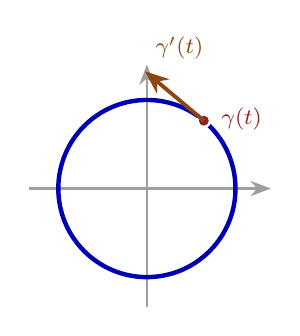
\begin{tikzpicture}[scale=0.75]
        \draw[axisln] (-2,0) -- (2.1,0);
        \draw[axisln] (0,-2) -- (0,2.1);
        \draw[curveln, blue!70!black] (0,0) circle (1.5);
        \dotpt{thmcolor}{({1.5*cos(50)},{1.5*sin(50)})}
        \draw[vec, mAccent] ({1.5*cos(50)},{1.5*sin(50)})
          -- ({1.5*cos(50)-1.3*sin(50)},{1.5*sin(50)+1.3*cos(50)});
        \node[mAccent, anchor=south] at (0.55,2.02) {\footnotesize $\gamma'(t)$};
        \node[thmcolor, anchor=west] at (1.1,1.17) {\footnotesize $\gamma(t)$};
      \end{tikzpicture}
      \end{center}
    \end{column}
    \begin{column}{0.64\textwidth}
      \begin{exblock}{Example: $\gamma(t) = (\cos t, \sin t)$, $0 \leq t \leq 2\pi$}
        $\gamma'(t) = (-\sin t, \cos t)$ is continuous, \\
        and $|\gamma'(t)| = \sqrt{\sin^2 t + \cos^2 t} = 1$.

        \vspace{0.2em}
        By Theorem 6.27:
        $\Lambda(\gamma) = \int_0^{2\pi} 1\,dt = 2\pi$.
      \end{exblock}

      \begin{exblock}{Same range, twice around}
        $\gamma_2(t) = (\cos 2t, \sin 2t)$, $0 \leq t \leq 2\pi$:
        $|\gamma_2'(t)| = 2$, so $\Lambda(\gamma_2) = \int_0^{2\pi} 2\,dt = 4\pi$.

        \vspace{0.2em}
        Length depends on the \alert{mapping}, not on the range.
      \end{exblock}
    \end{column}
  \end{columns}

  \note{
    Now take gamma sub 2 of "t" equals cosine of 2 "t" comma sine of 2
    "t", on the same parameter interval. Its range is the same unit
    circle, but the derivative picks up a factor of 2 from the chain
    rule: gamma sub 2 prime of "t" is minus 2 sine of 2 "t" comma 2
    cosine of 2 "t", whose absolute value is 2. So the speed is 2
    everywhere, and the integral from 0 to 2 pi of 2 is 4 pi. The moving point goes around the circle twice and
    travels twice the distance. This confirms concretely the remark we
    made earlier: the length is a property of the mapping gamma, not
    of the set of points it traces out. Two curves with the same range
    can have different lengths. Now let's prepare for the proof of the
    theorem.
  }
\end{frame}

% --- Build 1/2 ---
\begin{frame}{Recall: Two Tools from Section 4}
  \begin{thmblock}{Recall: Theorem 6.24 (Fundamental Theorem, vector version)}
    If $\mathbf{f} \in \mathscr{R}$ on $[a, b]$ and $\mathbf{F}' = \mathbf{f}$
    on $[a, b]$, then
    $\displaystyle \int_a^b \mathbf{f}(t)\,dt = \mathbf{F}(b) - \mathbf{F}(a)$.
  \end{thmblock}

  \begin{hlbox}
  Applied to $\mathbf{F} = \gamma$ on a subinterval $[x_{i-1}, x_i]$:
  $\displaystyle\; \gamma(x_i) - \gamma(x_{i-1}) = \int_{x_{i-1}}^{x_i} \gamma'(t)\,dt.$
  \end{hlbox}

  \note{
    The proof uses two results from the previous section, so let's
    recall them. The first is Theorem 6.24, the vector valued
    Fundamental Theorem of Calculus: if a vector function lowercase
    "f" is integrable and is the derivative of capital "F", then the
    integral of lowercase "f" from "a" to "b" is capital "F" of "b"
    minus capital "F" of "a". We apply it with capital "F" equal to
    gamma and lowercase "f" equal to gamma prime, which is integrable
    because it is continuous. On any subinterval from "x" sub "i" minus
    1 to "x" sub "i", the displacement gamma of "x" sub "i" minus gamma
    of "x" sub "i" minus 1 equals the integral of gamma prime over that
    subinterval. So each chord of the inscribed polygon is an integral
    of the velocity.
  }
\end{frame}

% --- Build 2/2 ---
\begin{frame}{Recall: Two Tools from Section 4}
  \begin{thmblock}{Recall: Theorem 6.24 (Fundamental Theorem, vector version)}
    If $\mathbf{f} \in \mathscr{R}$ on $[a, b]$ and $\mathbf{F}' = \mathbf{f}$
    on $[a, b]$, then
    $\displaystyle \int_a^b \mathbf{f}(t)\,dt = \mathbf{F}(b) - \mathbf{F}(a)$.
  \end{thmblock}

  \begin{hlbox}
  Applied to $\mathbf{F} = \gamma$ on a subinterval $[x_{i-1}, x_i]$:
  $\displaystyle\; \gamma(x_i) - \gamma(x_{i-1}) = \int_{x_{i-1}}^{x_i} \gamma'(t)\,dt.$
  \end{hlbox}

  \begin{thmblock}{Recall: Theorem 6.25 (triangle inequality for integrals)}
    If $\mathbf{f} \in \mathscr{R}(\alpha)$ on $[a, b]$, then
    $|\mathbf{f}| \in \mathscr{R}(\alpha)$ and
    $\displaystyle \Big|\int_a^b \mathbf{f}\,d\alpha\Big| \leq \int_a^b |\mathbf{f}|\,d\alpha$.
  \end{thmblock}

  \note{
    The second tool is Theorem 6.25, the triangle inequality for
    vector integrals: the absolute value of the integral of a vector
    function is at most the integral of its absolute value. In the
    previous episode we described this as displacement never exceeding
    distance traveled, and we proved it using the Schwarz inequality.
    Applied to gamma prime on a subinterval, it will tell us that each
    chord of the polygon is at most the integral of the speed over
    that subinterval. With these two tools in hand, here is the
    strategy of the proof.
  }
\end{frame}

% --- Build 1/3 ---
\begin{frame}{Proof Strategy: Theorem 6.27}
  \begin{hlbox}
  \textbf{Goal:} $\displaystyle \Lambda(\gamma) = \int_a^b |\gamma'(t)|\,dt$
  \quad (and in particular $\Lambda(\gamma) < \infty$)

  \vspace{0.4em}
  \textbf{Plan:} prove \alert{two inequalities}.

  \end{hlbox}
  \note{
    Our goal is the equality on the slide: the length of gamma equals
    the integral of the speed. Since the integral is a finite number,
    this equality includes the claim that gamma is rectifiable. As is
    typical for an equality between a supremum and something else, the
    plan is to prove two inequalities separately: the length is at
    most the integral, and the integral is at most the length. The two
    halves have quite different flavors.
  }
\end{frame}

% --- Build 2/3 ---
\begin{frame}{Proof Strategy: Theorem 6.27}
  \begin{hlbox}
  \textbf{Goal:} $\displaystyle \Lambda(\gamma) = \int_a^b |\gamma'(t)|\,dt$
  \quad (and in particular $\Lambda(\gamma) < \infty$)

  \vspace{0.4em}
  \textbf{Plan:} prove \alert{two inequalities}.
  \begin{enumerate}
    \item[($\leq$)] Each chord is at most the integral of the speed over its
      subinterval (Theorems 6.24 and 6.25); sum over $i$;\\
      take the sup over $P$.
  \end{enumerate}

  \end{hlbox}
  \note{
    The first half, the length is at most the integral, is the easy
    direction, and it follows directly from the two tools we just
    recalled. Each chord of an inscribed polygon is the absolute value
    of an integral of gamma prime, hence at most the integral of the
    absolute value of gamma prime over the same subinterval. Summing
    over the subintervals shows that every polygonal length is at most
    the full integral, and taking the supremum over all partitions
    gives the inequality for the length itself.
  }
\end{frame}

% --- Build 3/3 ---
\begin{frame}{Proof Strategy: Theorem 6.27}
  \begin{hlbox}
  \textbf{Goal:} $\displaystyle \Lambda(\gamma) = \int_a^b |\gamma'(t)|\,dt$
  \quad (and in particular $\Lambda(\gamma) < \infty$)

  \vspace{0.4em}
  \textbf{Plan:} prove \alert{two inequalities}.
  \begin{enumerate}
    \item[($\leq$)] Each chord is at most the integral of the speed over its
      subinterval (Theorems 6.24 and 6.25); sum over $i$;\\
      take the sup over $P$.
    \item[($\geq$)] Fix $\varepsilon > 0$. \alert{Uniform continuity} of
      $\gamma'$ gives a fine partition on which $\gamma'$ is nearly constant,
      so the integral of the speed over each subinterval is at most the chord
      plus $2\varepsilon\,\Delta x_i$. Sum, then let $\varepsilon \to 0$.
  \end{enumerate}

  \end{hlbox}
  \note{
    The second half, the integral is at most the length, is where the
    real work happens. Fix a small epsilon. Because gamma prime is
    continuous on a compact interval, it is uniformly continuous, so
    there is a mesh size below which gamma prime changes by less than
    epsilon across any subinterval. On such a fine partition the
    velocity is nearly constant on each piece, and the integral of the
    speed over the piece exceeds the chord by at most 2 epsilon times
    the width of the piece. Summing over the pieces bounds the whole
    integral by a polygonal length plus 2 epsilon times the length of
    the parameter interval, and letting epsilon go to zero finishes
    the proof. Let's carry out the first half.
  }
\end{frame}

% --- Build 1/3 ---
\begin{frame}{Proof --- Part 1: $\Lambda(\gamma) \leq \int_a^b |\gamma'(t)|\,dt$}
  \begin{proofblock}{Step 1: bound one chord}
    If $a \leq x_{i-1} < x_i \leq b$, then by Theorems 6.24 and 6.25,
    \[
      \textstyle |\gamma(x_i) - \gamma(x_{i-1})|
      = \Big| \int_{x_{i-1}}^{x_i} \gamma'(t)\,dt \Big|
      \leq \int_{x_{i-1}}^{x_i} |\gamma'(t)|\,dt.
    \]
  \end{proofblock}

  \note{
    Part 1 of the proof. Take any two consecutive points "x" sub "i"
    minus 1 and "x" sub "i" of a partition. By the Fundamental
    Theorem, Theorem 6.24, the displacement gamma of "x" sub "i" minus
    gamma of "x" sub "i" minus 1 equals the integral of gamma prime
    over the subinterval; this is the equality in the middle of the
    slide. By Theorem 6.25, the absolute value of that integral is at
    most the integral of the absolute value of gamma prime; this is
    the inequality on the right. The intuition is the one from the
    previous episode: the chord is the straight line displacement of
    the moving point over this time interval, and the integral of the
    speed is the distance it actually traveled, so the chord cannot be
    longer. Next we add these up.
  }
\end{frame}

% --- Build 2/3 ---
\begin{frame}{Proof --- Part 1: $\Lambda(\gamma) \leq \int_a^b |\gamma'(t)|\,dt$}
  \begin{proofblock}{Step 1: bound one chord}
    If $a \leq x_{i-1} < x_i \leq b$, then by Theorems 6.24 and 6.25,
    \[
      \textstyle |\gamma(x_i) - \gamma(x_{i-1})|
      = \Big| \int_{x_{i-1}}^{x_i} \gamma'(t)\,dt \Big|
      \leq \int_{x_{i-1}}^{x_i} |\gamma'(t)|\,dt.
    \]
  \end{proofblock}

  \begin{proofblock}{Step 2: sum over the subintervals}
    Hence, for \emph{every} partition $P$ of $[a, b]$,
    \[
      \textstyle \Lambda(P, \gamma) = \sum_{i} |\gamma(x_i) - \gamma(x_{i-1})|
      \leq \sum_{i} \int_{x_{i-1}}^{x_i} |\gamma'(t)|\,dt
      = \int_a^b |\gamma'(t)|\,dt.
    \]
  \end{proofblock}

  \note{
    Step 2: sum the chord bounds over all the subintervals of the
    partition. On the left we get the polygonal length Lambda of
    capital "P" and gamma. On the right we get the sum of the
    integrals of the speed over the subintervals, and by the additivity
    of the integral over adjacent intervals, Theorem 6.12 part "c",
    that sum is the integral of the speed over the whole interval from
    "a" to "b". Notice that the right side no longer depends on the
    partition: every inscribed polygon, no matter how fine, has length
    at most this one fixed number.
  }
\end{frame}

% --- Build 3/3 ---
\begin{frame}{Proof --- Part 1: $\Lambda(\gamma) \leq \int_a^b |\gamma'(t)|\,dt$}
  \begin{proofblock}{Step 1: bound one chord}
    If $a \leq x_{i-1} < x_i \leq b$, then by Theorems 6.24 and 6.25,
    \[
      \textstyle |\gamma(x_i) - \gamma(x_{i-1})|
      = \Big| \int_{x_{i-1}}^{x_i} \gamma'(t)\,dt \Big|
      \leq \int_{x_{i-1}}^{x_i} |\gamma'(t)|\,dt.
    \]
  \end{proofblock}

  \begin{proofblock}{Step 2: sum over the subintervals}
    Hence, for \emph{every} partition $P$ of $[a, b]$,
    \[
      \textstyle \Lambda(P, \gamma) = \sum_{i} |\gamma(x_i) - \gamma(x_{i-1})|
      \leq \sum_{i} \int_{x_{i-1}}^{x_i} |\gamma'(t)|\,dt
      = \int_a^b |\gamma'(t)|\,dt.
    \]
  \end{proofblock}

  \begin{proofblock}{Step 3: take the supremum over $P$}
    Sup over $P$:
    $\boxed{\textstyle \Lambda(\gamma) \leq \int_a^b |\gamma'(t)|\,dt < \infty}$,
    so $\gamma$ is \alert{rectifiable}.
  \end{proofblock}

  \note{
    Step 3: the integral of the speed is an upper bound for the set of
    all polygonal lengths, so it is at least their least upper bound,
    which is the length of gamma. That is the boxed inequality. Since
    the integral is a finite real number, the length is finite, so
    gamma is rectifiable. This already proves the first claim of the
    theorem. It remains to show that the integral is not bigger than
    the length, which is Part 2.
  }
\end{frame}

% --- Build 1/3 ---
\begin{frame}{Proof --- Part 2: Setup}
  \begin{proofblock}{Step 1: uniform continuity of $\gamma'$}
    Let $\varepsilon > 0$. Since $\gamma'$ is continuous on the compact
    set $[a, b]$, it is \alert{uniformly continuous} (Theorem 4.19):
    there is $\delta > 0$ such that
    $\; |\gamma'(s) - \gamma'(t)| < \varepsilon \;$ whenever $|s - t| < \delta$.
  \end{proofblock}

  \note{
    Part 2: we prove the opposite inequality, that the integral is at
    most the length. Let epsilon be a positive number. The function
    gamma prime is continuous on the closed interval "a" "b", which is
    compact, so by Theorem 4.19 it is uniformly continuous. This gives
    a positive delta with the property on the slide: whenever two
    parameter values "s" and "t" are within delta of each other, the
    velocity vectors gamma prime of "s" and gamma prime of "t" are
    within epsilon of each other. Uniformity is essential: the same
    delta works everywhere on the interval, which is what lets us
    choose a single partition that is fine enough for all
    subintervals at once.
  }
\end{frame}

% --- Build 2/3 ---
\begin{frame}{Proof --- Part 2: Setup}
  \begin{proofblock}{Step 1: uniform continuity of $\gamma'$}
    Let $\varepsilon > 0$. Since $\gamma'$ is continuous on the compact
    set $[a, b]$, it is \alert{uniformly continuous} (Theorem 4.19):
    there is $\delta > 0$ such that
    $\; |\gamma'(s) - \gamma'(t)| < \varepsilon \;$ whenever $|s - t| < \delta$.
  \end{proofblock}

  \begin{proofblock}{Step 2: choose a fine partition}
    Let $P = \{x_0, \dots, x_n\}$ be a partition of $[a, b]$ with
    $\Delta x_i < \delta$ for all $i$.
  \end{proofblock}

  \note{
    Step 2: choose a partition capital "P" of the interval, with
    points "x" sub 0 through "x" sub "n", such that every subinterval
    has width less than delta. Such partitions certainly exist; for
    instance, divide the interval into enough equal pieces. On each
    subinterval, any two parameter values are within delta of each
    other, so by Step 1 the velocity changes by less than epsilon
    across the subinterval. In other words, gamma prime is nearly
    constant on each piece.
  }
\end{frame}

% --- Build 3/3 ---
\begin{frame}{Proof --- Part 2: Setup}
  \begin{proofblock}{Step 1: uniform continuity of $\gamma'$}
    Let $\varepsilon > 0$. Since $\gamma'$ is continuous on the compact
    set $[a, b]$, it is \alert{uniformly continuous} (Theorem 4.19):
    there is $\delta > 0$ such that
    $\; |\gamma'(s) - \gamma'(t)| < \varepsilon \;$ whenever $|s - t| < \delta$.
  \end{proofblock}

  \begin{proofblock}{Step 2: choose a fine partition}
    Let $P = \{x_0, \dots, x_n\}$ be a partition of $[a, b]$ with
    $\Delta x_i < \delta$ for all $i$.
  \end{proofblock}

  \begin{proofblock}{Step 3: the speed is nearly constant on each piece}
    If $x_{i-1} \leq t \leq x_i$, then $|t - x_i| \leq \Delta x_i < \delta$, so
    $\; |\gamma'(t)| \leq |\gamma'(x_i)| + |\gamma'(t) - \gamma'(x_i)|
      < |\gamma'(x_i)| + \varepsilon.$
  \end{proofblock}

  \note{
    Step 3 records the consequence we need. Take any "t" in the
    subinterval from "x" sub "i" minus 1 to "x" sub "i". The distance
    from "t" to the right endpoint "x" sub "i" is at most the width of
    the subinterval, which is less than delta, so by Step 1 gamma
    prime of "t" is within epsilon of gamma prime of "x" sub "i". By the
    triangle inequality, the speed at time "t" is at most the speed at
    the right endpoint plus epsilon. So on each subinterval the speed
    is bounded by a constant, the speed at the right endpoint, up to an
    error of epsilon. Let's look at a picture of what this means
    before we do the key computation.
  }
\end{frame}

\begin{frame}{Proof --- Part 2: Why a Fine Partition Helps}
  \begin{center}
  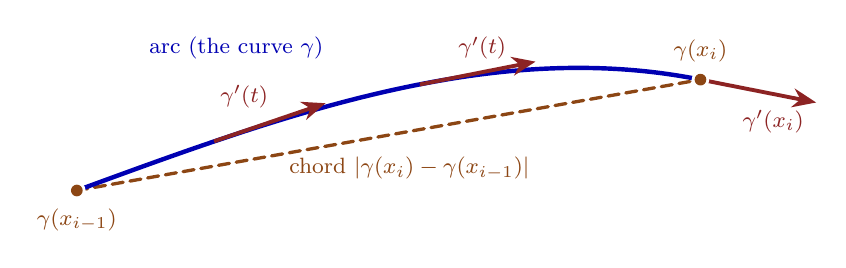
\begin{tikzpicture}[scale=0.88]
    % one piece of the curve: gently bowed, nearly straight
    \draw[chord, mAccent, dash pattern=on 4pt off 2.5pt] (0,0) -- (9,1.6);
    \draw[curveln, blue!70!black]
      (0,0) .. controls (3,1.1) and (6,2.2) .. (9,1.6);
    % velocity vectors (tangent, nearly equal), the last one at the right endpoint
    \draw[vec, thmcolor] (1.98,0.71) -- (3.59,1.26);
    \draw[vec, thmcolor] (4.95,1.53) -- (6.62,1.86);
    \draw[vec, thmcolor] (9,1.6) -- (10.67,1.27);
    \node[thmcolor, above left] at (2.9,1.05) {\footnotesize $\gamma'(t)$};
    \node[thmcolor, above] at (5.85,1.75) {\footnotesize $\gamma'(t)$};
    \node[thmcolor, below] at (10.05,1.3) {\footnotesize $\gamma'(x_i)$};
    % endpoints
    \dotpt{mAccent}{(0,0)}
    \dotpt{mAccent}{(9,1.6)}
    \node[mAccent, below] at (0,-0.12) {\footnotesize $\gamma(x_{i-1})$};
    \node[mAccent, above] at (9.0,1.72) {\footnotesize $\gamma(x_i)$};
    % labels for chord and arc
    \node[mAccent, below] at (4.8,0.62) {\footnotesize chord $|\gamma(x_i) - \gamma(x_{i-1})|$};
    \node[blue!70!black, above] at (2.3,1.75) {\footnotesize arc (the curve $\gamma$)};
  \end{tikzpicture}
  \end{center}

  \vspace{-0.6em}
  \begin{hlbox}
  \begin{center}
    \textcolor{thmcolor}{velocities nearly equal:}
    $|\gamma'(t) - \gamma'(x_i)| < \varepsilon$ for all $t \in [x_{i-1}, x_i]$,
    \\[0pt]
    \textcolor{mAccent}{so chord $\approx$ arc $\approx |\gamma'(x_i)|\,\Delta x_i$}
    \\[4pt]
    \textbf{Goal for one piece:}
    $\displaystyle \int_{x_{i-1}}^{x_i} |\gamma'(t)|\,dt
      \;\leq\; |\gamma(x_i) - \gamma(x_{i-1})| + 2\varepsilon\,\Delta x_i$
  \end{center}
  \end{hlbox}

  \note{
    This picture zooms in on a single subinterval of the fine
    partition. The blue arc is the piece of the curve from gamma of
    "x" sub "i" minus 1, the orange dot on the left, to gamma of "x"
    sub "i", the orange dot on the right, and the dashed orange
    segment is the chord joining these endpoints. The red arrows are
    velocity vectors: two of them, labeled gamma prime of "t", sit at
    interior times of the subinterval, and the third, at the right
    endpoint, is gamma prime of "x" sub "i". Because the partition is
    fine, these three vectors differ by less than epsilon, as the first
    line under the picture says: they are nearly parallel and nearly
    equal in length. So the curve is almost a straight segment
    traversed at almost constant velocity, and, as the second line
    says, the chord, the arc, and the product of the speed at the
    right endpoint with the time elapsed are all approximately equal.
    The goal at the bottom of the slide makes this precise: the
    integral of the speed over the piece exceeds the chord by at most
    2 epsilon times the width of the piece. Let's prove it.
  }
\end{frame}

% --- Build 1/4 ---
\begin{frame}{Proof --- Part 2: The Key Estimate on One Piece}
  \begin{proofblock}{Step 4: for the subinterval $[x_{i-1}, x_i]$}
    \begin{align*}
      \int_{x_{i-1}}^{x_i} |\gamma'(t)|\,dt
      &\leq |\gamma'(x_i)|\,\Delta x_i + \varepsilon\,\Delta x_i
    \end{align*}
  \end{proofblock}

  \begin{hlbox}
  {\small \textcolor{proofcolor}{Integrate the bound
  $|\gamma'(t)| \leq |\gamma'(x_i)| + \varepsilon$ from Step 3 over
  $[x_{i-1}, x_i]$.}}
  \end{hlbox}

  \note{
    Step 4 is the key estimate, and we build it one line at a time.
    The first line integrates the pointwise bound from Step 3 over the
    subinterval. The integrand is at most the constant absolute value
    of gamma prime of "x" sub "i" plus epsilon, and the integral of a
    constant over an interval is the constant times the width of the
    interval. So the integral of the speed over the piece is at most
    the speed at the right endpoint times the width, plus epsilon times
    the width. Next, we rewrite the first term as an integral so that
    we can compare it with the chord.
  }
\end{frame}

% --- Build 2/4 ---
\begin{frame}{Proof --- Part 2: The Key Estimate on One Piece}
  \begin{proofblock}{Step 4: for the subinterval $[x_{i-1}, x_i]$}
    \begin{align*}
      \int_{x_{i-1}}^{x_i} |\gamma'(t)|\,dt
      &\leq |\gamma'(x_i)|\,\Delta x_i + \varepsilon\,\Delta x_i \\
      &= \Big| \int_{x_{i-1}}^{x_i} \big[\gamma'(t) + \gamma'(x_i) - \gamma'(t)\big]\,dt \Big|
        + \varepsilon\,\Delta x_i
    \end{align*}
  \end{proofblock}

  \begin{hlbox}
  {\small \textcolor{proofcolor}{$\gamma'(x_i)$ is a \emph{constant vector}, so
  $|\gamma'(x_i)|\,\Delta x_i = \big|\int_{x_{i-1}}^{x_i} \gamma'(x_i)\,dt\big|$;\\
  then \alert{add and subtract $\gamma'(t)$} inside.}}
  \end{hlbox}

  \note{
    The second line is the trick of the proof. The vector gamma prime
    of "x" sub "i" is a constant, so its absolute value times the width
    of the subinterval is the absolute value of the integral of that
    constant vector over the subinterval. Inside that integral we add
    and subtract gamma prime of "t". This seems pointless, but look at
    what it sets up: the integrand is now the actual velocity gamma
    prime of "t" plus a small correction, gamma prime of "x" sub "i"
    minus gamma prime of "t". Since "t" and "x" sub "i" lie in the
    same short subinterval, Step 1 says that this correction has
    absolute value less than epsilon. Next we split the integral into
    these two parts.
  }
\end{frame}

% --- Build 3/4 ---
\begin{frame}{Proof --- Part 2: The Key Estimate on One Piece}
  \begin{proofblock}{Step 4: for the subinterval $[x_{i-1}, x_i]$}
    \begin{align*}
      \int_{x_{i-1}}^{x_i} |\gamma'(t)|\,dt
      &\leq |\gamma'(x_i)|\,\Delta x_i + \varepsilon\,\Delta x_i \\
      &= \Big| \int_{x_{i-1}}^{x_i} \big[\gamma'(t) + \gamma'(x_i) - \gamma'(t)\big]\,dt \Big|
        + \varepsilon\,\Delta x_i \\
      &\leq \Big| \int_{x_{i-1}}^{x_i} \gamma'(t)\,dt \Big|
        + \Big| \int_{x_{i-1}}^{x_i} \big[\gamma'(x_i) - \gamma'(t)\big]\,dt \Big|
        + \varepsilon\,\Delta x_i
    \end{align*}
  \end{proofblock}

  \begin{hlbox}
  {\small \textcolor{proofcolor}{Split the integral and use the
  \alert{triangle inequality} $|\mathbf{u} + \mathbf{v}| \leq |\mathbf{u}| + |\mathbf{v}|$.}}
  \end{hlbox}

  \note{
    The third line splits the integral in two, using linearity of the
    vector integral, and then applies the ordinary triangle inequality
    for vectors: the absolute value of a sum of two vectors is at most
    the sum of their absolute values. The first vector is the integral
    of the true velocity gamma prime of "t" over the piece, and the
    second is the integral of the small correction. Each of these has
    a clear meaning, and we bound them in the final line.
  }
\end{frame}

% --- Build 4/4 ---
\begin{frame}{Proof --- Part 2: The Key Estimate on One Piece}
  \begin{proofblock}{Step 4: for the subinterval $[x_{i-1}, x_i]$}
    \begin{align*}
      \int_{x_{i-1}}^{x_i} |\gamma'(t)|\,dt
      &\leq |\gamma'(x_i)|\,\Delta x_i + \varepsilon\,\Delta x_i \\
      &= \Big| \int_{x_{i-1}}^{x_i} \big[\gamma'(t) + \gamma'(x_i) - \gamma'(t)\big]\,dt \Big|
        + \varepsilon\,\Delta x_i \\
      &\leq \Big| \int_{x_{i-1}}^{x_i} \gamma'(t)\,dt \Big|
        + \Big| \int_{x_{i-1}}^{x_i} \big[\gamma'(x_i) - \gamma'(t)\big]\,dt \Big|
        + \varepsilon\,\Delta x_i \\
      &\leq |\gamma(x_i) - \gamma(x_{i-1})| + 2\varepsilon\,\Delta x_i.
    \end{align*}
  \end{proofblock}

  \begin{hlbox}
  {\small \textcolor{proofcolor}{First term: the \alert{chord} (Thm 6.24).
  Second: $\leq \varepsilon\,\Delta x_i$ (Thm 6.25 and Step 1).}}
  \end{hlbox}

  \note{
    The final line bounds the two pieces. The first integral, of gamma
    prime of "t" over the subinterval, is exactly the displacement
    gamma of "x" sub "i" minus gamma of "x" sub "i" minus 1 by the
    Fundamental Theorem, Theorem 6.24; its absolute value is the chord.
    For the second integral we use Theorem 6.25: its absolute value is
    at most the integral of the absolute value of the correction, and
    the correction is less than epsilon in absolute value throughout
    the subinterval, so this is at most epsilon times the width.
    Together with the epsilon times width already present, we get the
    chord plus 2 epsilon times the width of the subinterval. That is
    the goal we set for one piece. Now we add over all the pieces.
  }
\end{frame}

% --- Build 1/3 ---
\begin{frame}{Proof --- Part 2: Adding Up}
  \begin{proofblock}{Step 5: sum over $i = 1, \dots, n$}
    \begin{align*}
      \int_a^b |\gamma'(t)|\,dt
      &= \sum_{i=1}^{n} \int_{x_{i-1}}^{x_i} |\gamma'(t)|\,dt
      \leq \sum_{i=1}^{n} |\gamma(x_i) - \gamma(x_{i-1})| + 2\varepsilon \sum_{i=1}^{n} \Delta x_i \\
      &= \Lambda(P, \gamma) + 2\varepsilon\,(b - a)
    \end{align*}
  \end{proofblock}

  \note{
    Step 5: add the one piece estimates over all "n" subintervals. On
    the left, the integrals over the pieces add up to the integral of
    the speed over the whole interval. On the right, the chords add up
    to the polygonal length Lambda of capital "P" and gamma, and the
    widths of the subintervals add up to "b" minus "a", the length of
    the parameter interval. So the integral of the speed is at most
    the polygonal length plus 2 epsilon times "b" minus "a". Next we
    replace the polygonal length by the length of the curve.
  }
\end{frame}

% --- Build 2/3 ---
\begin{frame}{Proof --- Part 2: Adding Up}
  \begin{proofblock}{Step 5: sum over $i = 1, \dots, n$}
    \begin{align*}
      \int_a^b |\gamma'(t)|\,dt
      &= \sum_{i=1}^{n} \int_{x_{i-1}}^{x_i} |\gamma'(t)|\,dt
      \leq \sum_{i=1}^{n} |\gamma(x_i) - \gamma(x_{i-1})| + 2\varepsilon \sum_{i=1}^{n} \Delta x_i \\
      &= \Lambda(P, \gamma) + 2\varepsilon\,(b - a)
      \;\leq\; \Lambda(\gamma) + 2\varepsilon\,(b - a)
    \end{align*}
  \end{proofblock}

  \hl{\textcolor{proofcolor}{$\Lambda(P, \gamma) \leq \Lambda(\gamma)$ because
  $\Lambda(\gamma)$ is the supremum over all partitions.}}

  \note{
    Since the length of gamma is the supremum of the polygonal lengths
    over all partitions, the polygonal length for our particular
    partition capital "P" is at most Lambda of gamma. So the integral
    of the speed is at most the length of the curve plus 2 epsilon
    times "b" minus "a". Now recall that epsilon was an arbitrary
    positive number, chosen at the very start of Part 2, and the
    partition was chosen afterwards to suit it. The inequality holds
    for every epsilon.
  }
\end{frame}

% --- Build 3/3 ---
\begin{frame}{Proof --- Part 2: Adding Up}
  \begin{proofblock}{Step 5: sum over $i = 1, \dots, n$}
    \begin{align*}
      \int_a^b |\gamma'(t)|\,dt
      &= \sum_{i=1}^{n} \int_{x_{i-1}}^{x_i} |\gamma'(t)|\,dt
      \leq \sum_{i=1}^{n} |\gamma(x_i) - \gamma(x_{i-1})| + 2\varepsilon \sum_{i=1}^{n} \Delta x_i \\
      &= \Lambda(P, \gamma) + 2\varepsilon\,(b - a)
      \;\leq\; \Lambda(\gamma) + 2\varepsilon\,(b - a)
    \end{align*}
  \end{proofblock}

  \begin{proofblock}{Step 6: let $\varepsilon \to 0$}
    $\varepsilon$ was arbitrary:
    $\boxed{\textstyle \int_a^b |\gamma'(t)|\,dt \leq \Lambda(\gamma)}$.
    With Part 1: $\Lambda(\gamma) = \int_a^b |\gamma'(t)|\,dt$. \; $\blacksquare$
  \end{proofblock}

  \note{
    Step 6: since epsilon was arbitrary, the term 2 epsilon times "b"
    minus "a" can be made as small as we like, and we conclude that
    the integral of the speed is at most the length of gamma. This is
    the boxed inequality. Combined with Part 1, which gave the reverse
    inequality, we have equality: the length of gamma is the integral
    from "a" to "b" of the absolute value of gamma prime. This
    completes the proof of Theorem 6.27. Let's step back and review
    what we have learned.
  }
\end{frame}
}

{
\usebackgroundtemplate{%
  
\includegraphics[width=\paperwidth,height=\paperheight,keepaspectratio=false]{chapter_06_bg_05.png}%
}
\section{Summary}

% --- Build 1/3 ---
\begin{frame}{Summary}
  \begin{hlbox}
  \textbf{Key takeaways from this section:}
  \begin{itemize}
    \item \textbf{Definition 6.26:} a \alert{curve} is a continuous map
      $\gamma : [a, b] \to R^k$, a \emph{mapping}, not a set;
      one-to-one: \emph{arc}; $\gamma(a) = \gamma(b)$: \emph{closed curve}
  \end{itemize}

  \end{hlbox}
  \note{
    Let's review what we covered. First, Definition 6.26: a curve in
    "k" dimensional space is a continuous mapping from a closed
    interval into that space. It is the mapping that counts, not the
    set of points traced out: two different curves can have the same
    range, like the unit circle traversed once or twice. A one to one
    curve is an arc, and a curve that returns to its starting point is
    a closed curve. Next, length.
  }
\end{frame}

% --- Build 2/3 ---
\begin{frame}{Summary}
  \begin{hlbox}
  \textbf{Key takeaways from this section:}
  \begin{itemize}
    \item \textbf{Definition 6.26:} a \alert{curve} is a continuous map
      $\gamma : [a, b] \to R^k$, a \emph{mapping}, not a set;
      one-to-one: \emph{arc}; $\gamma(a) = \gamma(b)$: \emph{closed curve}
    \item \textbf{Length:} $\Lambda(\gamma) = \sup_P \Lambda(P, \gamma)$, the
      sup of \alert{inscribed polygon} lengths;
      \emph{rectifiable} means $\Lambda(\gamma) < \infty$ (not automatic!)
  \end{itemize}

  \end{hlbox}
  \note{
    Second, the length of a curve is defined geometrically: inscribe a
    polygon by choosing a partition of the parameter interval and
    joining the images of consecutive partition points, measure its
    length, and take the supremum over all partitions. Refining a
    partition never shortens the polygon, so the supremum is the
    natural limit. A curve is rectifiable when this supremum is
    finite, and we saw that continuity alone does not guarantee this:
    the curve "t" times sine of 1 over "t" is continuous but has
    infinite length. Finally, the main theorem.
  }
\end{frame}

% --- Build 3/3 ---
\begin{frame}{Summary}
  \begin{hlbox}
  \textbf{Key takeaways from this section:}
  \begin{itemize}
    \item \textbf{Definition 6.26:} a \alert{curve} is a continuous map
      $\gamma : [a, b] \to R^k$, a \emph{mapping}, not a set;
      one-to-one: \emph{arc}; $\gamma(a) = \gamma(b)$: \emph{closed curve}
    \item \textbf{Length:} $\Lambda(\gamma) = \sup_P \Lambda(P, \gamma)$, the
      sup of \alert{inscribed polygon} lengths;
      \emph{rectifiable} means $\Lambda(\gamma) < \infty$ (not automatic!)
    \item \textbf{Theorem 6.27:} $\gamma'$ continuous $\Rightarrow$ rectifiable,
      $\Lambda(\gamma) = \int_a^b |\gamma'(t)|\,dt$ (\emph{length $=$ integral
      of speed}); proof: Theorems 6.24, 6.25 $+$ \alert{uniform continuity}
  \end{itemize}

  \vspace{0.3em}
  \textbf{Coming up next:} Chapter 7, \alert{Sequences and Series of Functions}.

  \end{hlbox}
  \note{
    Third, Theorem 6.27: if gamma prime is continuous, then gamma is
    rectifiable and its length is the integral of the speed, the
    absolute value of gamma prime. In coordinates this is the arc
    length formula from calculus, now proved rather than assumed. The
    easy half, length at most the integral, came from the vector
    Fundamental Theorem and the triangle inequality for integrals:
    each chord is at most the corresponding piece of arc. The harder
    half used uniform continuity of gamma prime to make the velocity
    nearly constant on each piece of a fine partition, and an add and
    subtract trick to compare the integral of the speed with the
    chord. This concludes Chapter 6. In Chapter 7 we turn to sequences
    and series of functions, and ask when the limit of a sequence of
    functions inherits continuity, integrability, or differentiability
    from its terms. The answer, uniform convergence, will be one of the
    central ideas of analysis. See you next time.
  }
\end{frame}
}

\end{document}
